\documentclass[11,]{article}
\usepackage{lmodern}
\usepackage{amssymb,amsmath}
\usepackage{ifxetex,ifluatex}
\usepackage{fixltx2e} % provides \textsubscript
\ifnum 0\ifxetex 1\fi\ifluatex 1\fi=0 % if pdftex
  \usepackage[T1]{fontenc}
  \usepackage[utf8]{inputenc}
\else % if luatex or xelatex
  \ifxetex
    \usepackage{mathspec}
  \else
    \usepackage{fontspec}
  \fi
  \defaultfontfeatures{Ligatures=TeX,Scale=MatchLowercase}
\fi
% use upquote if available, for straight quotes in verbatim environments
\IfFileExists{upquote.sty}{\usepackage{upquote}}{}
% use microtype if available
\IfFileExists{microtype.sty}{%
\usepackage{microtype}
\UseMicrotypeSet[protrusion]{basicmath} % disable protrusion for tt fonts
}{}
\usepackage[margin=1in]{geometry}
\usepackage{hyperref}
\hypersetup{unicode=true,
            pdftitle={The information content of StockTwits},
            pdfauthor={Joyce Cahoon},
            pdfborder={0 0 0},
            breaklinks=true}
\urlstyle{same}  % don't use monospace font for urls
\usepackage{graphicx,grffile}
\makeatletter
\def\maxwidth{\ifdim\Gin@nat@width>\linewidth\linewidth\else\Gin@nat@width\fi}
\def\maxheight{\ifdim\Gin@nat@height>\textheight\textheight\else\Gin@nat@height\fi}
\makeatother
% Scale images if necessary, so that they will not overflow the page
% margins by default, and it is still possible to overwrite the defaults
% using explicit options in \includegraphics[width, height, ...]{}
\setkeys{Gin}{width=\maxwidth,height=\maxheight,keepaspectratio}
\IfFileExists{parskip.sty}{%
\usepackage{parskip}
}{% else
\setlength{\parindent}{0pt}
\setlength{\parskip}{6pt plus 2pt minus 1pt}
}
\setlength{\emergencystretch}{3em}  % prevent overfull lines
\providecommand{\tightlist}{%
  \setlength{\itemsep}{0pt}\setlength{\parskip}{0pt}}
\setcounter{secnumdepth}{0}
% Redefines (sub)paragraphs to behave more like sections
\ifx\paragraph\undefined\else
\let\oldparagraph\paragraph
\renewcommand{\paragraph}[1]{\oldparagraph{#1}\mbox{}}
\fi
\ifx\subparagraph\undefined\else
\let\oldsubparagraph\subparagraph
\renewcommand{\subparagraph}[1]{\oldsubparagraph{#1}\mbox{}}
\fi

%%% Use protect on footnotes to avoid problems with footnotes in titles
\let\rmarkdownfootnote\footnote%
\def\footnote{\protect\rmarkdownfootnote}

%%% Change title format to be more compact
\usepackage{titling}

% Create subtitle command for use in maketitle
\newcommand{\subtitle}[1]{
  \posttitle{
    \begin{center}\large#1\end{center}
    }
}

\setlength{\droptitle}{-2em}

  \title{The information content of StockTwits}
    \pretitle{\vspace{\droptitle}\centering\huge}
  \posttitle{\par}
    \author{Joyce Cahoon}
    \preauthor{\centering\large\emph}
  \postauthor{\par}
    \date{}
    \predate{}\postdate{}
  
\usepackage{placeins}
\usepackage{chngcntr}
\usepackage{multicol}
\usepackage{setspace}
\usepackage{mathrsfs}
\usepackage{amsthm}
\usepackage{graphicx}
\usepackage{booktabs}
\usepackage{multirow}
\usepackage{subcaption}
\usepackage{sidecap}
\usepackage{mathtools}
\usepackage{bm}
\usepackage[linesnumbered,algoruled,boxed,lined,commentsnumbered]{algorithm2e}
\SetKwInput{KwInput}{Input}
\SetKwInput{KwOutput}{Output}
\onehalfspacing
\setlength{\parskip}{8.0pt}
\newcommand{\V}[1]{{\bm{#1}}}
\newcommand{\Real}{\mathbb{R}}
\newcommand{\Exp}{\mathbb{E}}
\newcommand{\ubar}[1]{\underbar{$#1$}}
\newcommand{\obar}{\overline}
\newtheorem{walley781}{Theorem}
\usepackage[symbols,nogroupskip,nonumberlist,automake]{glossaries-extra}
\makeglossaries
\newglossaryentry{T}{name=\ensuremath{T}, description={Number of topics},type=symbols}

\begin{document}
\maketitle
\begin{abstract}
blah
\end{abstract}

{
\setcounter{tocdepth}{2}
\tableofcontents
}
\newpage

\hypertarget{introduction}{%
\section{Introduction}\label{introduction}}

As fund managers, we were tasked with constructing a cross-sectional,
long-short US equity strategy on
\href{https://www.quantopian.com/}{Quantopian}. There were not many
explicit constraints on the specific strategy we utilized, but it must
pass the following criteria: (i) trade liquid stocks, (ii) have no more
than 5\% of capital invested in any one asset, (iii) have no more than
10\% net dollar exposure, (iv) achieve mean daily turnover between 5\%
and 65\% over a 63-trading-day rolling window, (v) attain gross leverage
between 0.8x and 1.1x, (vi) have low correlation to the market, (vii)
have less than 20\% exposed to each of the 11 sectors as defined on
Quantopian, and (viii) result in positive returns. While the last return
criteria was not a constraint we included in our optimization, we did
design our algorithm with the rest of the seven criteria in mind
(Quantopian \protect\hyperlink{ref-q}{2018}).

The algorithm I eventually submitted was one based purely on the
information content from StockTwits; more specifically, the 5-day moving
average of the bull minus bear intensity associated with each tradable
stock. I rely on this metric to assign each stock's weight in our
portfolio, subject to certain constraints so that our algorithm passes
\texttt{Quantopian}'s criteria to remain in competition. Given the large
literature around news and social media sentiment in driving volatility
and liquidity in the market, I wanted to examine the power of this
unstructured data in driving returns.

My algorithm's performance over the November period resulted in a final
rank of 105 out of 261 submissions and a total score of 0.338. Its
performance is mediocre at best and can be attributed the fact that the
tuning mechanism for my input parameters was based only on the backtest
returns. Given the constraints and the length of moving window for our
sentiment metric was overfit to a backtest window between 2016 and 2018,
my strategy may have experienced bad out-of-sample performance.

Nevertheless, this strategy did perform within the top 40\% of all
submissions, which corroborates many findings in literature that social
media has some effect on driving prices. The majority of literature
suggests extreme sentiment or extreme volume of online media content
tends to drive the positive and negative returns, and since the month of
November can be characterized by extreme volatility this may explain the
high performance of our sentiment strategy. As expected, for December,
the peaks in the VIX, however, have subsided given greater clarity
around the Trump administration's trade policy and Fed's decision to
stop raising rates, and our strategy fell a few ranks to 113 with a
score of 0.316 (Gurdus \protect\hyperlink{ref-cramer2018}{2018}).

\hypertarget{related-work}{%
\section{Related Work}\label{related-work}}

The first paper that explored the relationship of text---unstructured
data---in driving stock prices was Cutler et al.
(\protect\hyperlink{ref-cutler1988}{1988})'s ``What moves stock
prices?'' At the time, the field of computational linguistics was yet
sophisticated enough to process large collections of text, so Cutler and
his team examined 49 major events discussed in the NY Times Business
desk and assessed the market changes associated with each event.
Unfortunately, given the number of significant market moves associated
with days where nothing significant was released, they were unable to
identify any link between market moves and news, possibly stymeing
explorations into this realm (Cutler et al.
\protect\hyperlink{ref-cutler1988}{1988}). Fortunately, another
empirical study emerged in 1998, which leveraged information on online
message boards instead, identifying strong correlations between stocks
with high message volume and high market valuation. In fact, Wysocki
found message volume forecasted not only abnormal stock returns the next
day, but also trading volume the next day (Wysocki
\protect\hyperlink{ref-wysocki1998}{1998}).

Yet, given these results and similar findings from papers like Bagnoli
et al. (\protect\hyperlink{ref-bagnoli1999}{1999}), Antweiler and Frank
(\protect\hyperlink{ref-antweiler2004}{2004}), corroborating the link
between prices and social chatter, a number of studies find the
opposite. Tumarkin and Whitelaw
(\protect\hyperlink{ref-tumarkin2001}{2001}) found no relationship for
equities in the tech sector and the message activity on RagingBull.com.
Das and Chen (\protect\hyperlink{ref-das2007}{2007}) developed a
classifier for investor sentiment from message board text, yet were
unable to to demonstrate its ability to forecast returns. Dewally
(\protect\hyperlink{ref-dewally2003}{2003}) found recommendations
exchanged on sites like \texttt{misc.invest.stocks} and
\texttt{alt.invest.penny-stocks} had no effect on the return
characteristics of the stocks under discussion.

Despite these mixed claims, newer studies arose reporting the opposite.
In fact, the seminar paper by Tetlock
(\protect\hyperlink{ref-tetlock2007}{2007}) concluded high negative
sentiment in the Wall Street Journal predicted temporary downward price
pressure, echoing the thoughts expressed in Wysocki
(\protect\hyperlink{ref-wysocki1998}{1998}) that extreme news affects
market movement. Additional works that build on Tetlock's use of news as
a fundamental factor is Mitra et al.
(\protect\hyperlink{ref-mitra2008}{2008}), Leinweber and Sisk
(\protect\hyperlink{ref-leinweber2011}{2011}) and Fang and Peress
(\protect\hyperlink{ref-fang2009}{2009}), each providing evidence for
the predictive value in social chatter. In this class, we were also
directed to the paper by Agrawal et al.
(\protect\hyperlink{ref-agrawal2019}{2019}), which provides a great
overview of literature that further promotes the use of Twitter and
StockTwits to predict stock volatility, liquidity and return.

\hypertarget{our-reliance-on-stocktwits}{%
\section{Our Reliance on StockTwits}\label{our-reliance-on-stocktwits}}

Key to my strategy is the output from the \texttt{bull\_minus\_bear} API
call as it is this signal that is fed into the optimization function and
this result that determines the order size of each asset. While there is
no disclosure on the natural language processing model that calculates
the bull and bear intensity of each social media message, it is helpful
to look at examples and understand the nature of posts that ultimately
determine the power of our sentiment measure as shown in Figure
\ref{StockT}.

\begin{figure}

{\centering 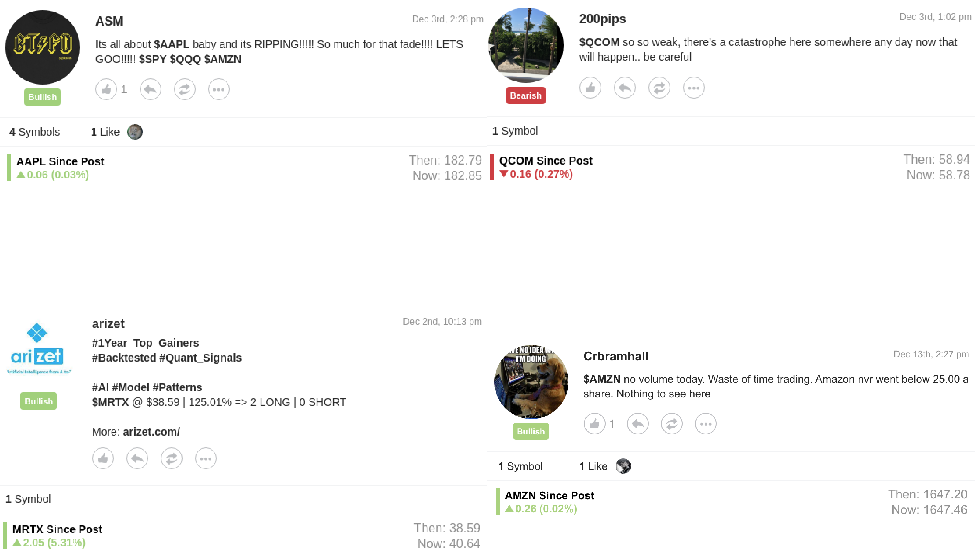
\includegraphics[width=0.8\linewidth]{cahoon_final_paper_files/figure-latex/unnamed-chunk-2-1} 

}

\caption{\label{StockT}Four examples of messages posted on StockTwits. The bull and bear indicator is provided by the user, and all stock tickers that follow the cashtag is associated with this indicator. The bull and bear intensity is then computed by a proprietary StockTwits algorithm based on the content within each individual post.}\label{fig:unnamed-chunk-2}
\end{figure}

While we do not have exact clarity on the natural language processing
engine that calculates the bullish intensity and bearish intensity of a
stock, we do know how the \texttt{bull\_minus\_bear} signal arises;
traders attached either a bull emoji or a bear emoji to any message they
release on the \texttt{StockTwits} platform as well as a ticker symbol
that identifies which asset is under discussion. While traders attached
a clear label to the asset of interest, \texttt{StockTwits} also has an
in-house proprietary algorithm that processes some of the language in
the message to ascribe an intensity level of the bull or bear indicator.
Messages across the \texttt{StockTwits} platform is thus aggregated to
arrive a sentiment score that is a function of subtracting the bearish
intensity from the bullish intensity result.

In addition to the ease of implementation, we chose to rely on the
sentiment factor as it seems to have some good characteristics, namely:

\begin{enumerate}
\def\labelenumi{\arabic{enumi}.}
\item
  \textbf{Predictive alpha} We calculated the mean information
  coefficient using the built-in function in \texttt{alphalens} and
  found our sentiment signal matches the direction of actual asset
  returns. As shown in the top-left of the figure below, we only get the
  full exposure of this factor 5 days after this signal becomes
  available. In fact, prior to 5 trading days, it appears the signal
  hurts us, in that its forecast is negative. Counterintuitively, after
  we cross 5 trading days, it appears our sentiment factor gains more
  predictive power. This is further corroborated in the top-right graph
  in that returns are highest when the signal is delayed by four days.
  Given this characteristic, we may want to build greater exposure to
  this factor since it still benefits us after 10 trading days. We can
  also leverage the positive effects of this factor by increasing our
  turnover constraints as it appears it does not hurt our portfolio to
  keep in there for a longer period of time. Nevertheless, the mean
  information coefficient across the time frame displayed still lingers
  around 0, suggesting the forecasting benefits provided by our
  sentiment factor may be no better than the results we get from
  randomly selecting our asset weights.
\item
  \textbf{Low exposures} We quantified the exposures via the
  \texttt{perf\_attrib} function in \texttt{pyfolio}. As shown in the
  bottom-left, our sentiment factor appears to have relatively low
  exposures throughout, with most of the returns from volatility risk.
  However, there does appear to be persistent exposure to value and
  short term reversal, in that it is shifted to the left of zero; and
  persistent exposure to size and momentum, in that it is shifted to the
  right of zero. Ideally, we would choose a factor that doesn't display
  this skew, but the skew does not appear too large. We also benefit
  from the fact that the width of each of our box and whisker plots are
  not that wide, so our exposures do not vary much over time. Yet, this
  analysis was conducted only over the available sentiment signal in
  2018, so there may be other extended periods prior to 2018 in which
  our factor over or underperforms. Given what we have here, we may want
  to identify asset classes to include in our portfolio that would
  offset the exposure risks identified above.
\end{enumerate}

Unfortunately, when we examine our exposures through cumulative returns
and volatility, we find that our sentiment factor may not be as strong
as we desired. As shown by the left bar graph (bottom-right), most of
our returns are obtained from exposure to common risk factors, and, as
shown in the right bar graph, are in fact driven by these common risk
factors. Ideally, we would like to strip away the contribution from
these common risk factors as portfolio performance from this exposure
can easily be replicated from ETFs or other easy, cost-effective
methods.

\hypertarget{trading-strategy}{%
\section{Trading Strategy}\label{trading-strategy}}

Section 4 should be~Trading-Strategy Analysis. This is the major section
of the whole paper. You should give a detailed description of
your~procedure. I prefer you use mathematical/statistical
modeling/formulas as much as you can, instead of sampling quoting
~generic functions' description provided in quantopian. Discussions
about why your method will not violate contest constraints, why your
method performs good (or not so good) should be included.~

\hypertarget{backtest-analysis}{%
\section{Backtest Analysis}\label{backtest-analysis}}

Section 5 should be about the Backtest Analysis. You need to summarize
details on the backtesting procedure and results provided in quantopian.
You should try to interpret and relate your results with domain
knowledge.~

\hypertarget{performance}{%
\section{Performance}\label{performance}}

Section 6 should be a summary about your performance in the contest.
Again you~need to summarize the results provided in quantopian. You
should try to interpret and relate your results with domain knowledge.~

\hypertarget{discussion}{%
\section{Discussion}\label{discussion}}

Section 7 will be the conclusion and discussion. You may revisit the
advantage and disadvantage of your strategy and provide some insights
for future exploration directions.~ In the appendix, all your programing
codes should be attached.~

\hypertarget{python-code}{%
\section{Python Code}\label{python-code}}

\hypertarget{references}{%
\section*{References}\label{references}}
\addcontentsline{toc}{section}{References}

\hypertarget{refs}{}
\leavevmode\hypertarget{ref-agrawal2019}{}%
Agrawal, S., Azar, P., Lo, A., and Singh, T. (2019), ``Practical
applications of momentum, mean-reversion, and social media: Evidence
from stocktwits and twitter,'' \emph{Practical Applications},
Institutional Investor Journals Umbrella, 6, 1--4.

\leavevmode\hypertarget{ref-antweiler2004}{}%
Antweiler, W., and Frank, M. (2004), ``Is all that talk just noise? The
information content of internet stock message boards,'' \emph{The
Journal of finance}, Wiley Online Library, 59, 1259--1294.

\leavevmode\hypertarget{ref-bagnoli1999}{}%
Bagnoli, M., Beneish, M., and Watts, S. (1999), ``Whisper forecasts of
quarterly earnings per share,'' \emph{Journal of Accounting and
Economics}, Elsevier, 28, 27--50.

\leavevmode\hypertarget{ref-cutler1988}{}%
Cutler, D., Poterba, J., and Summers, L. (1988), ``What moves stock
prices?'' National Bureau of Economic Research.

\leavevmode\hypertarget{ref-das2007}{}%
Das, S., and Chen, M. (2007), ``Yahoo! For amazon: Sentiment extraction
from small talk on the web,'' \emph{Management science}, INFORMS, 53,
1375--1388.

\leavevmode\hypertarget{ref-dewally2003}{}%
Dewally, M. (2003), ``Internet investment advice: Investing with a rock
of salt,'' \emph{Financial Analysts Journal}, CFA Institute, 59, 65--77.

\leavevmode\hypertarget{ref-fang2009}{}%
Fang, L., and Peress, J. (2009), ``Media coverage and the cross-section
of stock returns,'' \emph{The Journal of Finance}, Wiley Online Library,
64, 2023--2052.

\leavevmode\hypertarget{ref-cramer2018}{}%
Gurdus, E. (2018), ``Cramer: Volatility charts suggest now is the time
to buy into stocks,'' \emph{CNBC},
\url{https://www.cnbc.com/2018/11/27/cramer-volatility-charts-suggest-now-is-the-time-to-buy-into-stocks.html}.

\leavevmode\hypertarget{ref-leinweber2011}{}%
Leinweber, D., and Sisk, J. (2011), ``Event driven trading and the'new
news'.''

\leavevmode\hypertarget{ref-mitra2008}{}%
Mitra, L., Mitra, G., and Bartolomeo, D. (2008), ``Equity portfolio risk
(volatility) estimation using market information and sentiment,''
\emph{Quantitative Finance}.

\leavevmode\hypertarget{ref-q}{}%
Quantopian (2018), \url{https://www.quantopian.com/contest}.

\leavevmode\hypertarget{ref-tetlock2007}{}%
Tetlock, P. (2007), ``Giving content to investor sentiment: The role of
media in the stock market,'' \emph{The Journal of finance}, Wiley Online
Library, 62, 1139--1168.

\leavevmode\hypertarget{ref-tumarkin2001}{}%
Tumarkin, R., and Whitelaw, R. (2001), ``News or noise? Internet
postings and stock prices,'' \emph{Financial Analysts Journal}, CFA
Institute, 57, 41--51.

\leavevmode\hypertarget{ref-wysocki1998}{}%
Wysocki, P. (1998), ``Cheap talk on the web: The determinants of
postings on stock message boards.''


\end{document}
